\section{Poissonness plot}\label{sec:discrete-Poissonness}
\ix{Poissonness plot|(}

The Poissonness plot
\citep{Hoaglin:80}
is designed as a plot of some
quantity against \(k\), so that the result will be points along a
straight line when the data follow a \IX{Poisson distribution}.  When the
data deviate from a Poisson, the points will be curved.
\citet{HoaglinTukey:85}
develop similar plots for other discrete distributions,
including the binomial, negative binomial, and logarithmic series
distributions.
\ix{binomial distribution}
\ix{negative binomial distribution}

\subsection{Features of the Poissonness plot}
The Poissonness plot has the following desirable features:
\begin{itemize}
\item \boldital{Resistance}: a single discrepant value of \(n_k\)
       affects only the point at value \(k\).  (In the Ord plot
       it affects each of its neighbors.)
\item \boldital{Comparison standard}:  An approximate confidence
       interval can be found for each point, indicating its inherent
       variability and helping to judge whether each point is
       discrepant.
\item \boldital{Influence}:  Extensions of the method result in
       plots which show the effect of each point on the estimate of
       the main parameter of the distribution (\(\lambda\) in the
       Poisson).
\end{itemize}

\subsection{Plot construction}
Assume, for some fixed \(\lambda\), each observed frequency, \(n_k\)
equals the expected frequency, \(m_k = N p_k\).  Then, setting
\(n_k = N p_k  = N { e^{ - \lambda } \:  \lambda^k } /  { k ! }\),
and taking logs of both sides gives

\begin{equation*}
  \log ( n_k ) = \log \,  N - \lambda  +  k \,  \log \,  \lambda  -
  \log \,  k !
\end{equation*}
which can be rearranged to
\begin{equation} \label{eq:poispl}
  \log \left(  \frac{ k ! \:  n_k } {N} \right)
 = - \lambda  +  ( \log \,  \lambda ) \,  k
 \period
\end{equation}

The left side of \eqref{eq:poispl} is called the \glossterm{count metameter}, and
denoted \(\phi \,  ( n_k )  = \log_e ( k ! \,  n_k  /  N )\).  Hence,
plotting \(\phi ( n_k )\) against \(k\) should give a line
\(\phi ( n_k )= a + b k\) with

\begin{itemize*}
\item slope = \(\log  \,  \lambda\)
\item intercept = \(- \lambda\)
\end{itemize*}
when the observed frequencies follow a Poisson distribution.
If the points in this plot are close enough to a straight line,
then an estimate of $\lambda$ may be obtained from the slope $b$ of the line,
$\hat{\lambda} = e^b$ should be reasonably close in value
to the MLE of $\lambda$, $\hat{\lambda} = \bar{x}$.
In this case, we might as well use the MLE as our estimate.

\subsubsection{Leveled plot}
If we have a preliminary estimate $\lambda_0$ of $\lambda$,
we can use this to give a new plot where the reference line
is horizontal, making comparison of the points with the line
easier.
In this leveled plot the vertical coordinate $\phi (n_k)$ is modified to
\begin{equation*}
 \phi ' (n_k) = \phi (n_k) + \lambda_0 - k \log \lambda_0
 \period
\end{equation*}
When the data follow a Poisson distribution with parameter
$\lambda$, the modified plot will have
\begin{itemize*}
\item slope = \(\log  \lambda - \log  \lambda_0 = \log ( \lambda / \lambda_0 ) \)
\item intercept = \(\lambda_0 - \lambda\)
\end{itemize*}
In the ideal case, where our estimate of $\lambda_0$ is close to the true
$\lambda$, the line will be horizontal at $\phi ' = 0$.
The modified plot is particularly useful in conjunction with the
confidence intervals for individual points described below.

\subsubsection{Confidence intervals}
When one or two points deviate from an otherwise nearly linear
relation,
it is helpful to determine whether the discrepancy is consistent with
chance variation.
As well, we must recognize that classes with small frequencies $n_k$
are less precise than classes with large frequencies.
\citet{HoaglinTukey:85} develop approximate confidence intervals
for $\log m_k$ for each point in the Poissonness plot.
These are calculated as
\begin{equation*}
\phi \left( n_k^{*}\right) \pm h_k
\end{equation*}
where the count metameter function is calculated using a modified frequency $%
n_k^{*}$, defined as

\begin{equation*}
n_k^{*}= \left\{
\begin{array}{ll}
n_k-.8n_k-.67 & n\geq 2 \\
1/e & n=1 \\
\textrm{undefined} & n=0
\end{array}
\right.
\end{equation*}
%
and $h_k$ is the half-width of the 95\% confidence interval,
\begin{equation*}
h_k=1.96\frac{\sqrt{1-\widehat{p}_k}}{[n_k-(.25\widehat{p}_k+.47)\sqrt{n_k}%
]^{1/2}}
\end{equation*}
and $\hat{p}_k = n_k / N$.

\subsection{The \macro{POISPLOT}}
The \macro{POISPLOT} (see \macref{mac:poisplot}) performs the calculations and produces the
plots for all examples shown in this section.
The input data should contain a basic count variable (corresponding to $k$)
and a frequency variable (corresponding to $n_k$)
of the form shown in \tabref{tab:horskick}.

\begin{Example}[horskick2]{Death by horse kick}
A Poissonness plot is produced for the Horse kick data
using the \macro{POISPLOT} with
the following statements:
\begin{listing}
title 'Poissoness Plot: Deaths by Horsekicks' ;
data horskick;
    input deaths corpsyrs;
    label deaths='Number of Deaths'
       corpsyrs='Number of Corps-Years';
   datalines;
    0    109
    1     65
    2     22
    3      3
    4      1
;
%poisplot(data=horskick, count=Deaths,freq=corpsyrs);

\end{listing}

The calculations for the poissonness plot, including confidence
intervals, are shown below for the horse kicks data.  The macro
produces the plot in
\figref{fig:poisdemo1}.
The fitted least squares line has a slope of -0.431, which would
indicate $\lambda = e^{-0.431} = 0.65$.  This compares well with the MLE,
$\lambda = \bar{x} = 0.61$.
\ixd{death by horse kick}

\begin{alltt}
           \(\phi(n\sb{k})\)        CI       CI      Confidence Int
k    nk        Y       center   width     lower    upper

0   109   -0.607      -0.617    0.130    -0.748   -0.487
1    65   -1.124      -1.138    0.207    -1.345   -0.931
2    22   -1.514      -1.549    0.417    -1.966   -1.132
3     3   -2.408      -2.666    1.318    -3.984   -1.348
4     1   -2.120      -3.120    2.689    -5.809   -0.432
\end{alltt}
\begin{figure}[htb]
  \centering
  \includegraphics[scale=.5]{poisdemo1}\graphicsfile{ch2/fig/poisdemo1.eps}{}
  \caption[Poissonness plots for the horse kick data]{Poissonness plots
for the horse kick data.  The data fits the Poisson distribution
reasonably well.}\label{fig:poisdemo1}
\end{figure}

The leveled Poissonness plot (see \figref{fig:poisdemo2}) is produced by the \texttt{\%POISPLOT} statement
below, specifying \pname{LAMBDA=.610}.
%% input: /users/faculty/friendly/sasuser/catdata/poisdemo.sas
%% last modified: 08-Apr-99 12:38
\begin{listing}
title;
%poisplot(data=horskick, count=Deaths, freq=corpsyrs,
          lambda=.610, plot=dist);
run;
\end{listing}

\begin{figure}[htb]
  \centering
  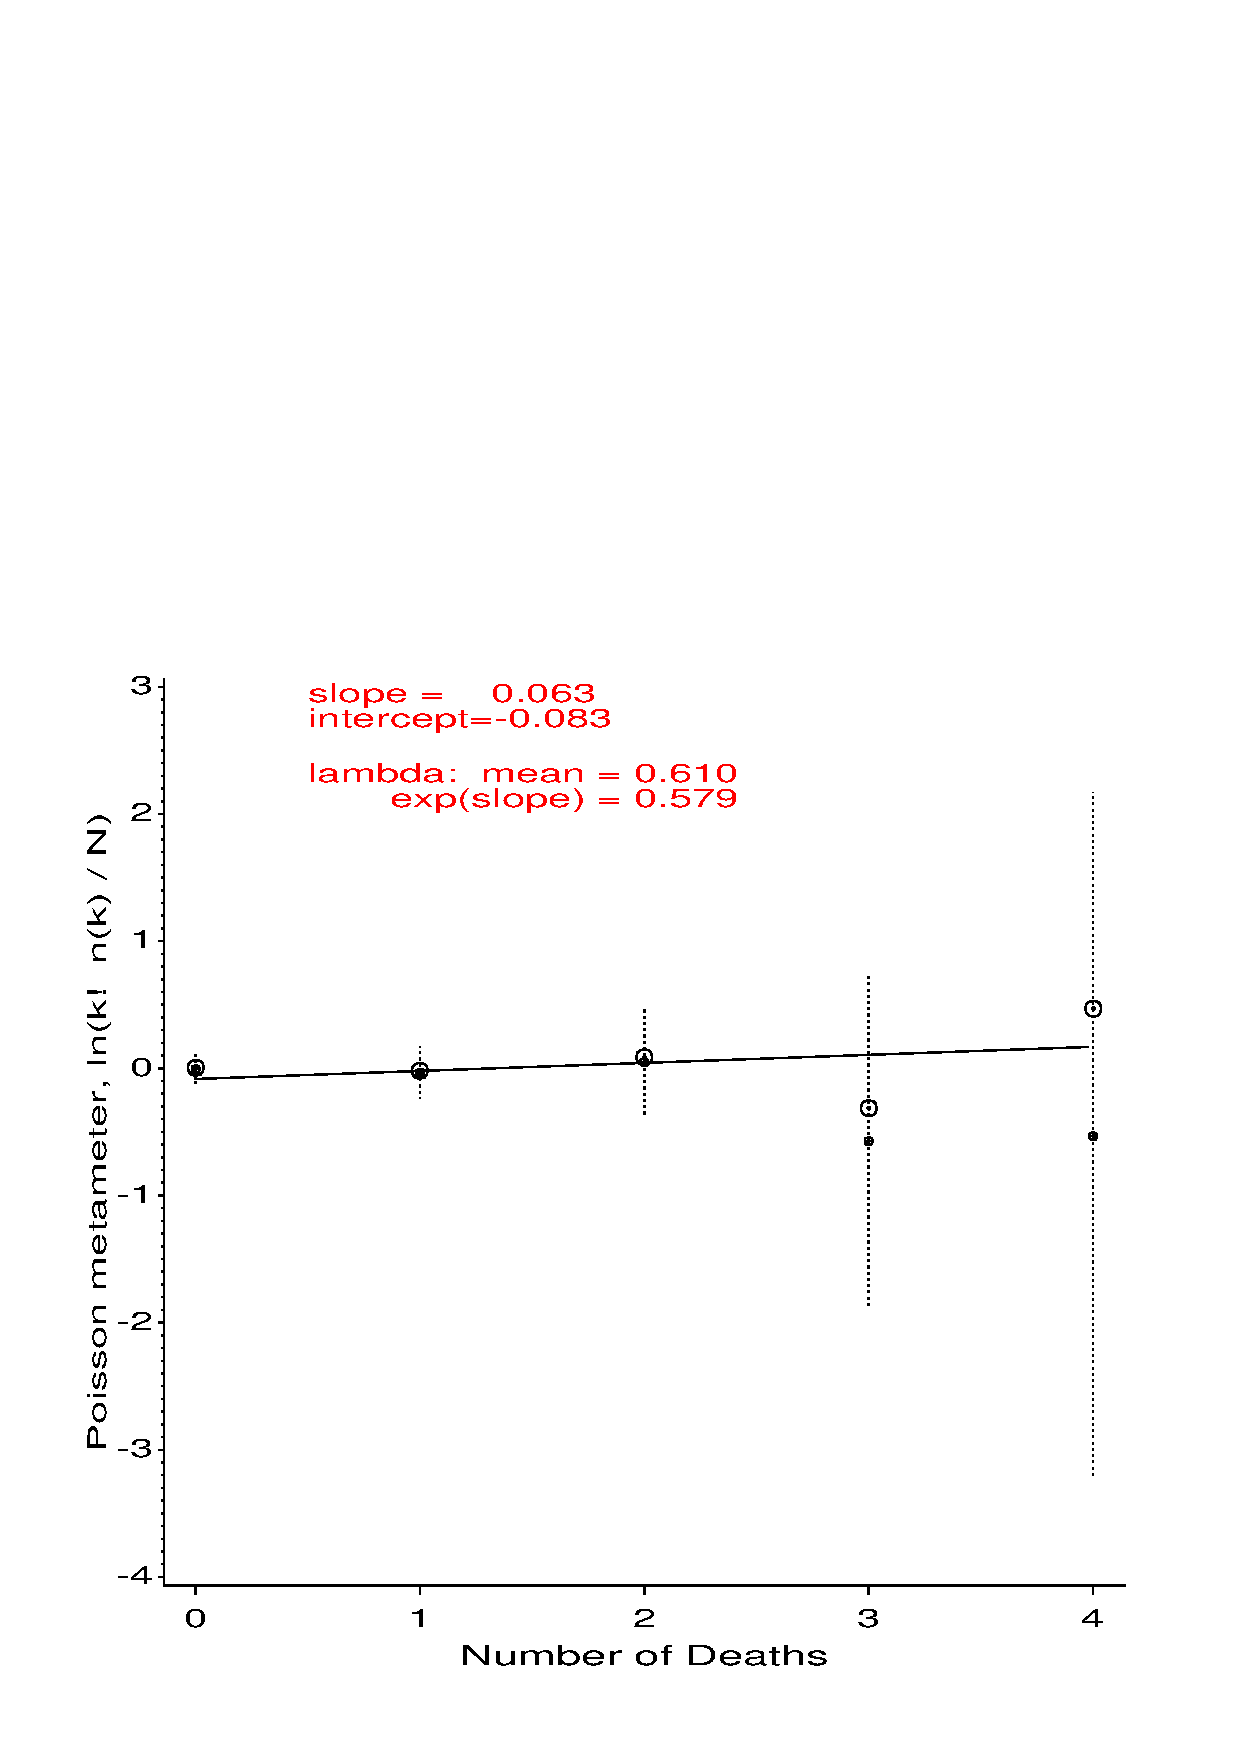
\includegraphics[scale=.5]{poisdemo2}\graphicsfile{ch2/fig/poisdemo2.eps}{}
  \caption[Leveled poissonness plot for the horse kick data]{Leveled poissonness plot for the horse kick data.}\label{fig:poisdemo2}
\end{figure}
In both plots the fitted line is within the confidence intervals;
the widths of the intervals for $k > 2$ are graphic reminders that these observations
have relatively low precision.

For comparison, \figref{fig:poismad1} shows the Poissonness plot
for the occurrences of \emph{may} in the
Federalist Papers (\tabref{tab:madison}).
The systematic curvature in the plot, judged relative to the confidence
intervals,
 indicates that these data do not follow a Poisson distribution.
\end{Example}

\begin{figure}[htb]
  \centering
  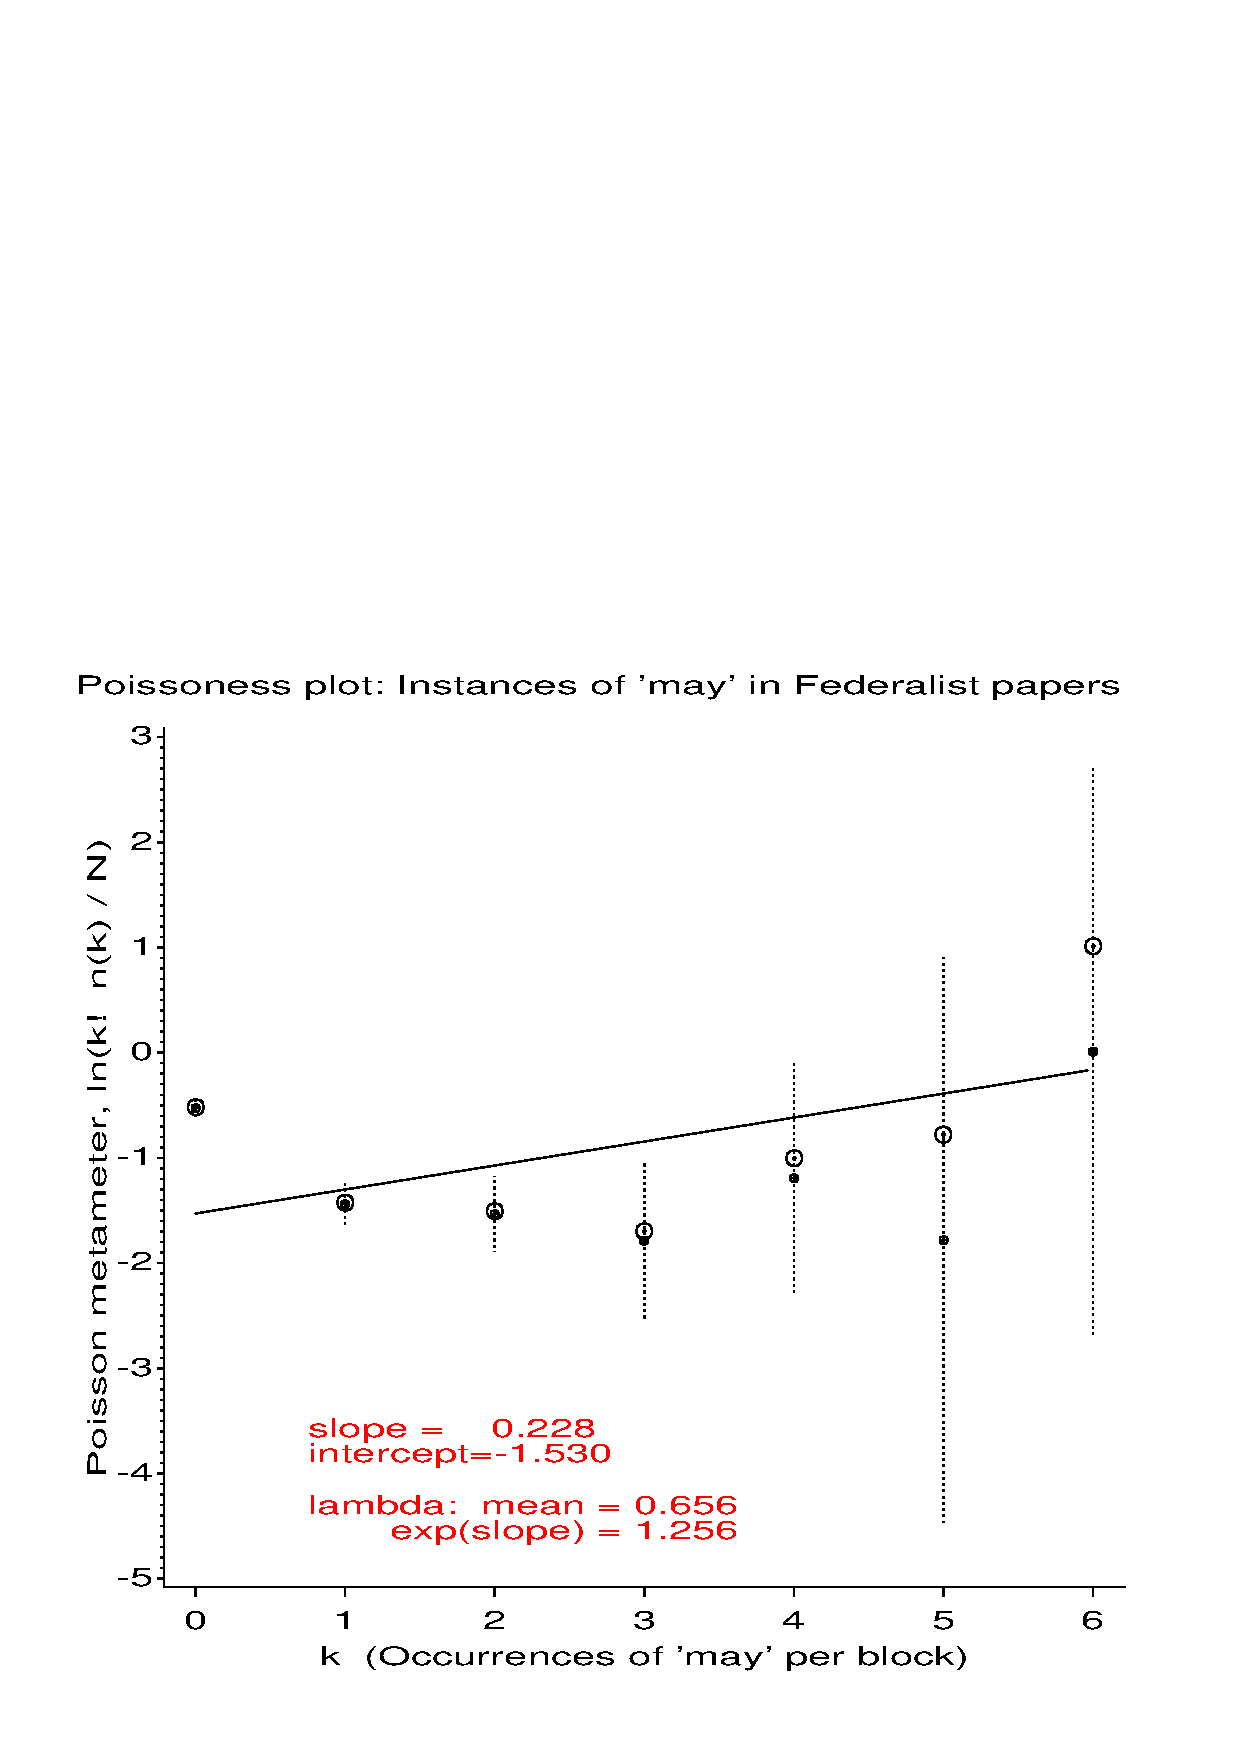
\includegraphics[scale=.5]{poismad1}\graphicsfile{ch2/fig/poismad1.eps}{}
  \caption[Poissonness plot for the Federalist Papers data]{Poissonness plot for the Federalist Papers data.
The systematic curvature in the plot indicates that this data does not follow a Poisson distribution.}\label{fig:poismad1}

\end{figure}
\subsection{Leverage and influence}
In standard models for quantitative data, common diagnostic techniques
attempt to estimate the effect that each observation has upon the
parameter estimates.
For linear models, these include measures of
\glossterm{leverage}---the potential
that an observation has to influence our results (due to its location
on the predictors),
and \glossterm{influence}---the actual effect this observation has
on parameter estimates and fitted values.

For discrete distributions, \citet{HoaglinTukey:85} derive
measures which are similar in spirit,  though based on the change in
the estimate of $ \lambda$ at each value of $k$ which would be
required to make the observed count metameter $\phi(n_k^{*})$
equal to its fitted value,
$\phi(m_k(\lambda_0))$ calculated using a contemplated or estimated $ \lambda_0$.

For the Poisson distribution, their analysis leads to the relation
\begin{equation}\label{eq:levpois}
\log \frac{\phi(n_k^{*})}{\phi(m_k(\lambda_0))}
= ( \lambda - \lambda_0 ) \left( \frac{k}{\lambda_0} - 1 \right)
\period
\end{equation}
Equation \eqref{eq:levpois} is 
a line through the origin with slope equal to $( \lambda - \lambda_0 )$.
By analogy with least squares regression through the origin
(where leverage is proportional to $x$), Hoaglin and Tukey
refer to $(k/\lambda_0) - 1$ as the leverage of point $k$.

Their parameter change plot shows each observation in the discrete
distribution as a point with vertical coordinate proportional to
$ \log [ \phi(n_k^{*}) / \phi(m_k(\lambda_0)) ] =
  \log ( \phi(n_k^{*})) - \log \phi(m_k(\lambda_0))$
and horizontal coordinate proportional to $k/\lambda_0 - 1$.
In this plot (see \figref{fig:poisdemo3}), the slope of
a line from the origin to a point shows the change in the Poisson
parameter, $\lambda - \lambda_0$ indicated by that
point.
The horizontal coordinate is proportional to the potential
of that observation to affect the Poisson parameter $\lambda$.

An alternative version of this plot, more in the spirit of the
influence plots for \loglin{} models and logistic regression
to be described later in this book, plots the
parameter change, $\lambda - \lambda_0$ directly on the
vertical axis against the same horizontal leverage value,
and uses a bubble whose size represents influence
as the plotting symbol.
%[More to be added here]

The parameter change plot and the influence plot are produced
with the \macro{POISPLOT} by including the keyword
\texttt{INFL} in the \texttt{PLOT=} parameter (i.e., \texttt{PLOT=DIST INFL}
gives all plots).
For the horse kick data, these plots are shown in
\figref{fig:poisdemo3} and \figref{fig:poisdemo4}.

\begin{figure}[htb]
  \centering
  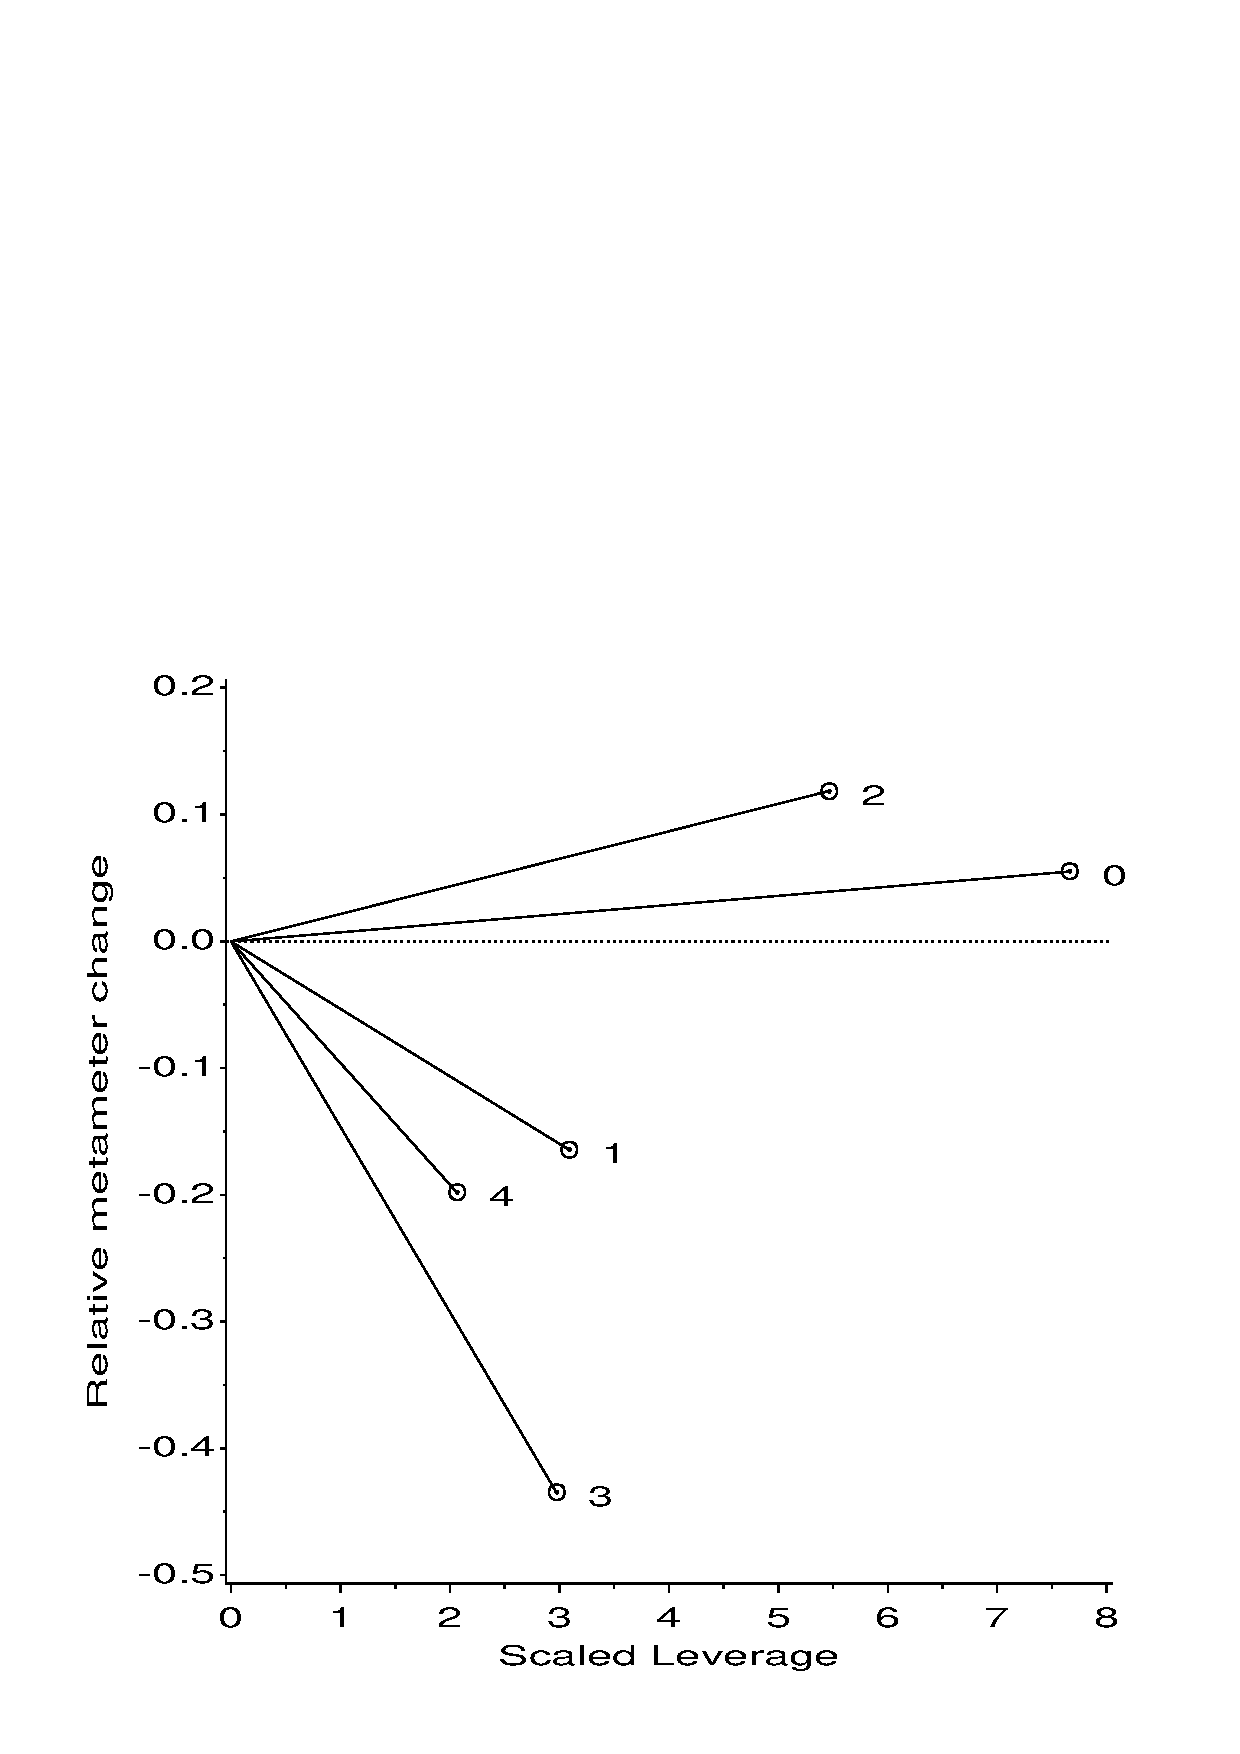
\includegraphics[scale=.5]{poisdemo3}\graphicsfile{ch2/fig/poisdemo3.eps}{}
  \caption[Parameter change plot for the Poisson parameter]{Parameter change
plot for the Poisson parameter, fitting the horse kick data.
The horizontal coordinate of each point is proportional to the potential of that observation to affect the value of $\lambda$.
The slope of the line through the origin is proportional to the
change in the count metameter.}\label{fig:poisdemo3}
\end{figure}
In \figref{fig:poisdemo3} we see that
the point corresponding to $k=0$ has the greatest leverage, but
influences $\lambda$ very little.
The point for $k=3$ has only moderate leverage, but has the greatest
impact on the Poisson parameter.
In \figref{fig:poisdemo2}
we see that the circle symbol for $\phi(n_k^{*})$
at $k=3$ is furthest from the
line.
\figref{fig:poisdemo4} shows that this point indicates a $\lambda$
value about 0.15 smaller than the estimated value.
\begin{figure}[htb]
  \centering
  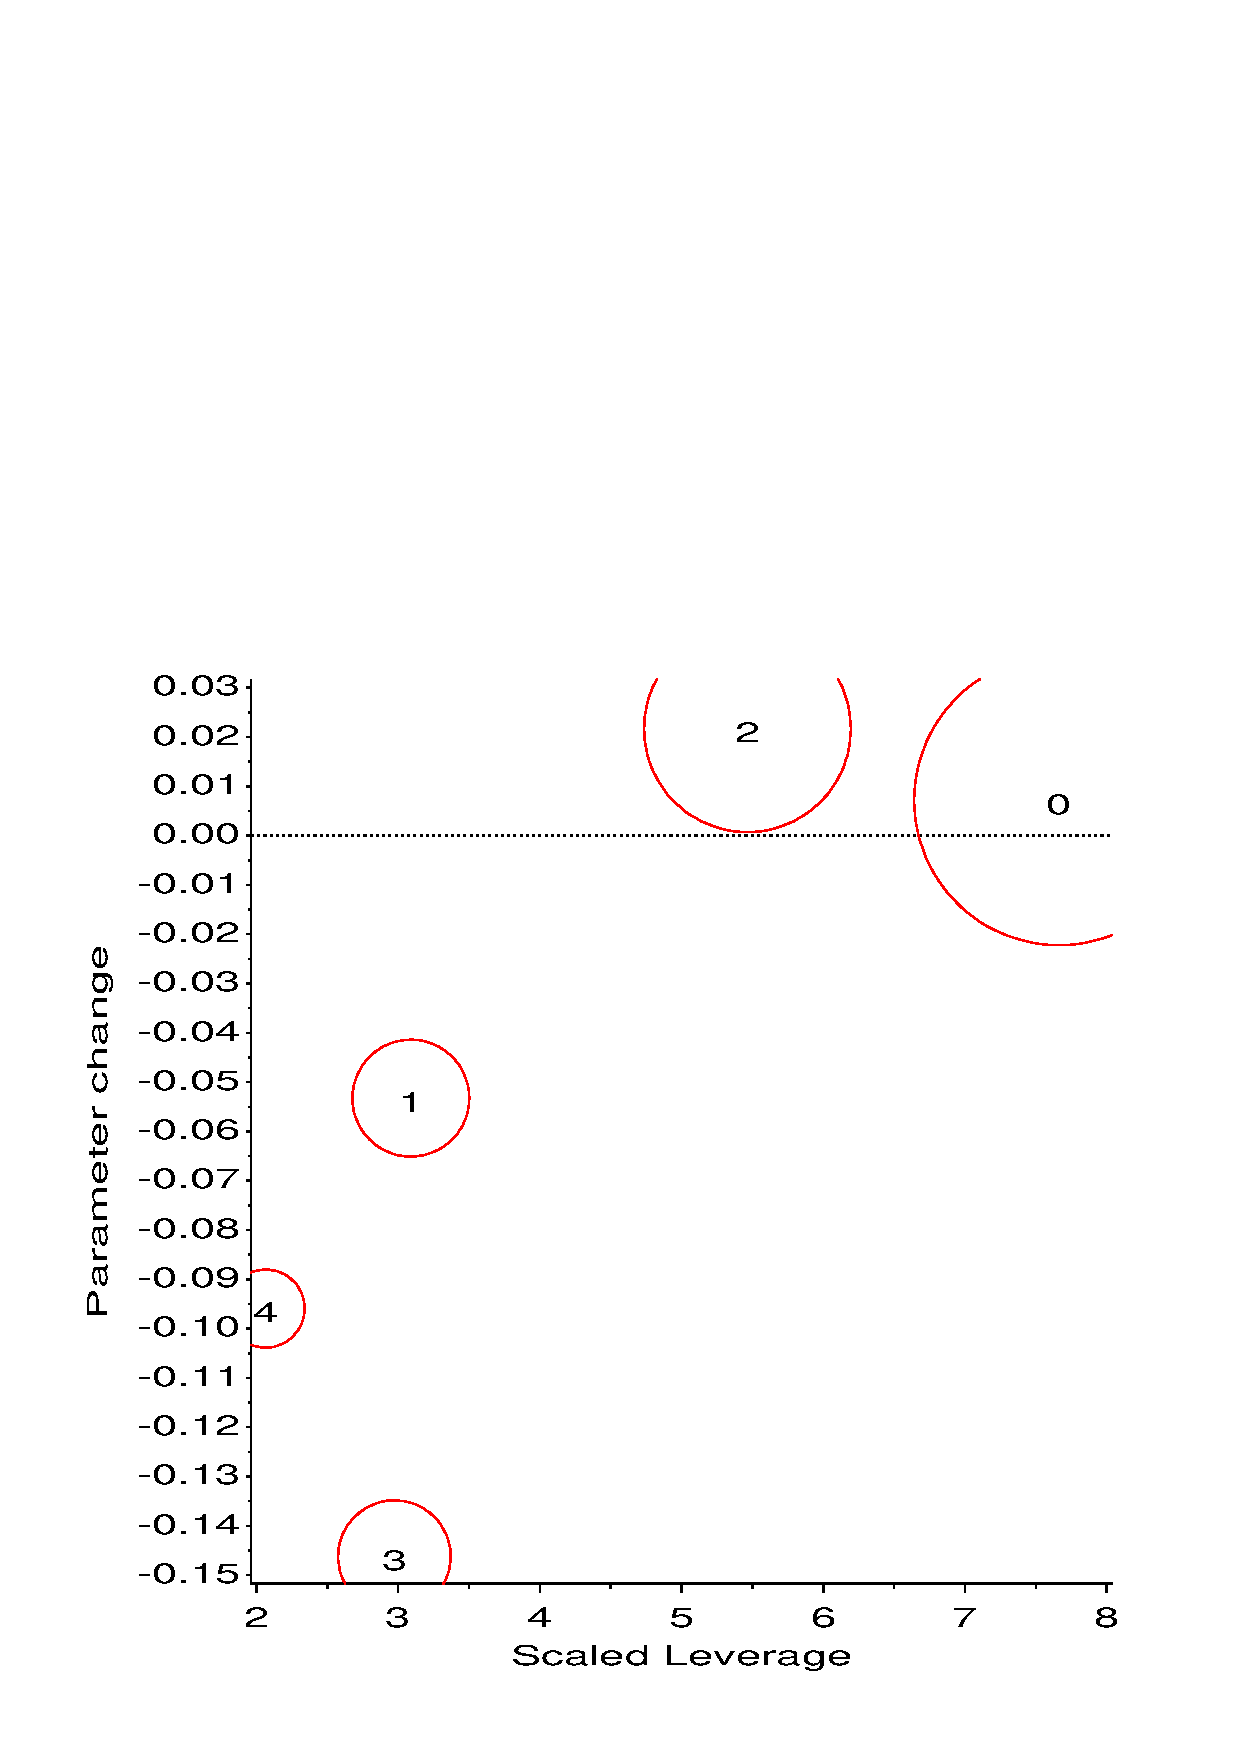
\includegraphics[scale=.5]{poisdemo4}\graphicsfile{ch2/fig/poisdemo4.eps}{}
  \caption[Influence plot for the Poisson parameter]{Influence plot
for the Poisson parameter, fitting the horse kick data.
  The ordinate shows the indicated change in $\lambda$
directly, and the bubble size is proportional to
influence.}\label{fig:poisdemo4} \end{figure}


\ix{Poissonness plot|)}

\subsection{Plots for other distributions}\label{sec:discrete-other}
As described in \secref{sec:pwrseries}, the binomial, Poisson, negative binomial,
geometric, and logseries distributions are all members of the
general  power series family of discrete distributions.
For this family, \citet{HoaglinTukey:85} develop similar plots
of a count metameter against $k$ which appear as a straight line
when a data distribution follows a given family member.

The distributions which can be analyzed in this way are shown in
\tabref{tab:distparms}, with the interpretation given to the
slope and intercept in each case.
For example, for the Binomial distribution, a ``binomialness''
plot is constructed by plotting $\log n_k^{*} / N \binom{n}{k}$
against $k$.  If the points in this plot approximate a straight
line, the slope is interpreted as $\log (p/(1-p))$, so the
binomial parameter $p$ may be estimated as $p = e^b/(1+e^b)$.
\begin{table}[!b]
\caption[Plot parameters for five discrete distributions]{Plot parameters for five discrete distributions. In each case the count metameter, $\phi
(n_k^{*})$ is plotted against $k$, yielding a straight line when the data
follow the given distribution.}
\label{tab:distparms}
 \begin{center}
\begin{tabular}{p{2.4cm}llll}
  \hline
  \tableheader
%              & Probability      & Count                      & Theoretical & Theoretical \\
%Distributiion & function, $p(k)$ & metameter, $\phi(n_k^{*})$ & Slope ($b$) & Intercept ($a$)\\[1ex]
  \multilineL{Distribution\\} & \multilineL{Probability\\function, $p(k)$} & \multilineL{Count)\\metameter, $\phi(n_k^{*})$} & \multilineL{Theoretical\\ slope ($b$)} &
  \multilineL{Theoretical\\ intercept ($a$)} \\
  \hline \\[.3ex]
Poisson          & $e^{-\lambda }\lambda ^k/k!$ & $\log (k!n_k^{*}/N)$ & $\log
(\lambda )$ & -$\lambda $ \\[.7ex]
%
Binomial          & $\binom nkp^k(1-p)^{n-k}$ & $\log \left( n_k^{*}/N\binom
nk\right) $ & $\log \left(\frac{p}{1-p}\right)$ & $n\log (1-p)$ \\[.7ex]
%
Negative binomial & $\binom{n+k-1}kp^n(1-p)^k$ & $\log \left( n_k^{*}/N%
\binom{n+k-1}k\right) $ & $\log (1-p)$ & $n\log (p)$ \\[.7ex]
%
Geometric         & $p(1-p)^k$ & $\log \left( n_k^{*}/N\right) $ & $\log (1-p)$ & $\log (p)$ \\[.7ex]
%
Log series        & $\theta ^k/[-k\log (1-\theta )]$ & $\log \left(
kn_k^{*}/N\right) $ & $\log (\theta )$ & $-\log \left( -\log (1-\theta)\right) $ \\[1ex]%
  \hline
  \multicolumn{5}{p{\textwidth}}{\emph{Source}: adapted from \citet{HoaglinTukey:85}, Table 9-15.} \\
\end{tabular}
 \end{center}
\end{table}



Unlike the Ord plot, a different plot is required for each distribution,
because the count metameter, \(\phi ( n_k )\), differs
from distribution to distribution.
Moreover, systematic deviation from a linear relationship does not
       indicate which distribution provides a better fit.
However, the attention to robustness, and the availability of confidence
intervals and influence diagnostics make this a highly useful tool
for visualizing discrete distributions.


\subsubsection{\macro{DISTPLOT}}
The \macro{DISTPLOT} (see \macref{mac:distplot}) carries out the analysis and produces overall
distribution plots and influence plots for the members of the
power series distributions shown in \tabref{tab:distparms}.
As with the \macro{GOODFIT} values for parameters for a given distribution
may be supplied
in the \mparm{PARM}{DISTPLOT}.

When the value of the distribution parameter
is not supplied, the macro produces the overall distribution plot
whose slope $b$ (and intercept $a$) are used to find graphical
estimates of the parameter.
For most distributions, the available MLE or moments estimates
given in \secref{sec:discrete-distrib}
are also calculated and displayed in the plot.
When the value of the distribution parameter is supplied,
a leveled plot is produced, with graphical parameter estimates adjusted
for the leveling.

\begin{Example}[saxony3]{Families in Saxony}
Our analysis in \exref{ex:saxony1} and \exref{ex:saxony2} of
the Saxony data
showed that the distribution of male children had slightly heavier tails
than the binomial.
We can see this even more clearly in the distribution diagnostic
plot produced
by the \macro{DISTPLOT}.  For a binomial distribution, we might call
this a ``binomialness plot''.

\figref{fig:saxony1} is produced with the statement
\begin{listing}
%distplot(data=saxony, count=males, freq=families, dist=binomial);
\end{listing}
The systematic curvature of the points again indicates the inadequacy
of the binomial, and the widths of the intervals around the points
show that the two extreme points are of limited reliability.
Comparing this plot with the hanging rootogram (\figref{fig:saxony}),
we see that heavy-tailed distributions will tend to curve upwards.
We also see that the estimate of $p = \exp(b) / [1+\exp(b)] $ from the slope of the fitted
line is quite close to the maximum likelihood estimate.
\begin{figure}[htb]
  \centering
  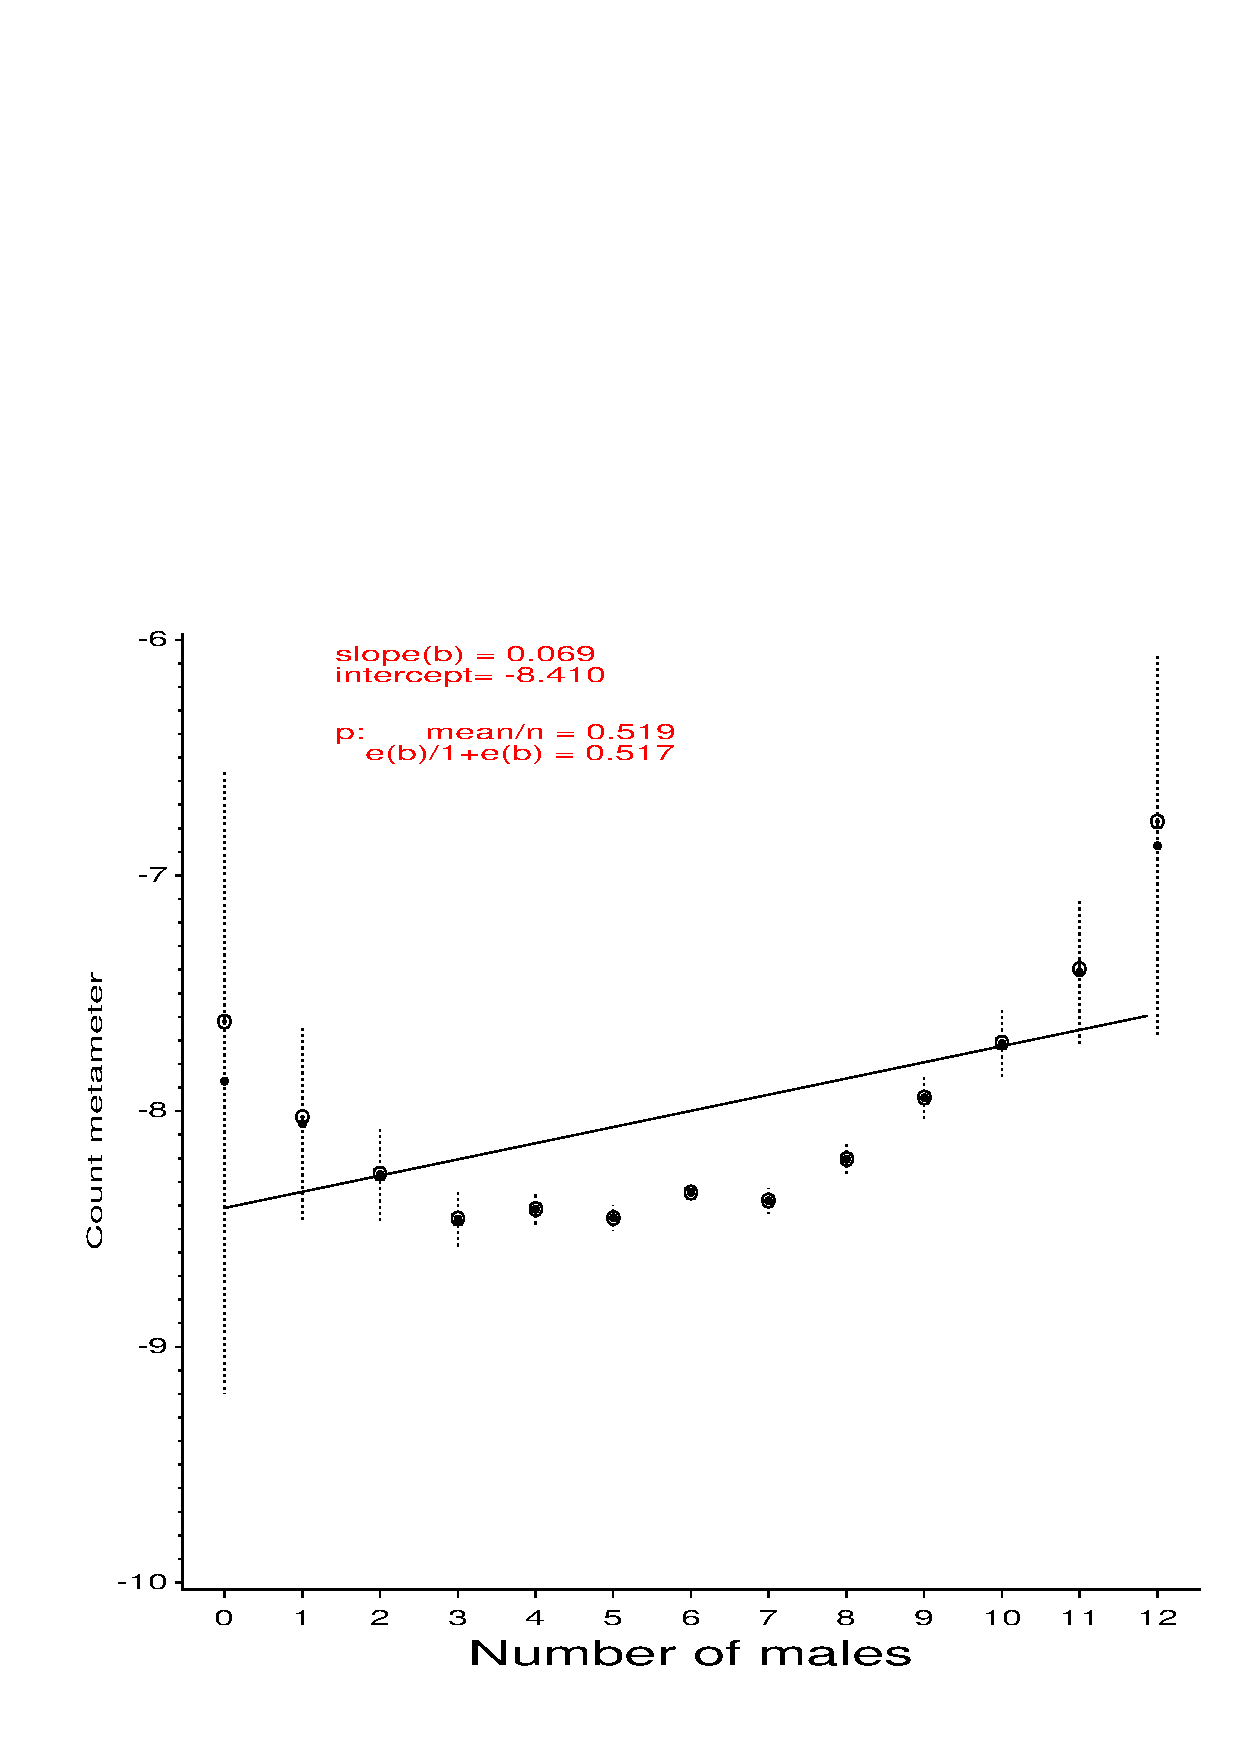
\includegraphics[scale=.6]{saxony1}\graphicsfile{ch2/fig/saxony1.eps}{}
  \caption{Binomialness plot for the distribution of males in Saxony families. }%
  \label{fig:saxony1}
\end{figure}
\end{Example}
